\documentclass{standalone}
\usepackage{tikz}
\usetikzlibrary{patterns, positioning}
\usepackage[sfdefault]{ClearSans} %% option 'sfdefault' activates Clear Sans as the default text font
\usepackage[T1]{fontenc}

\begin{document}
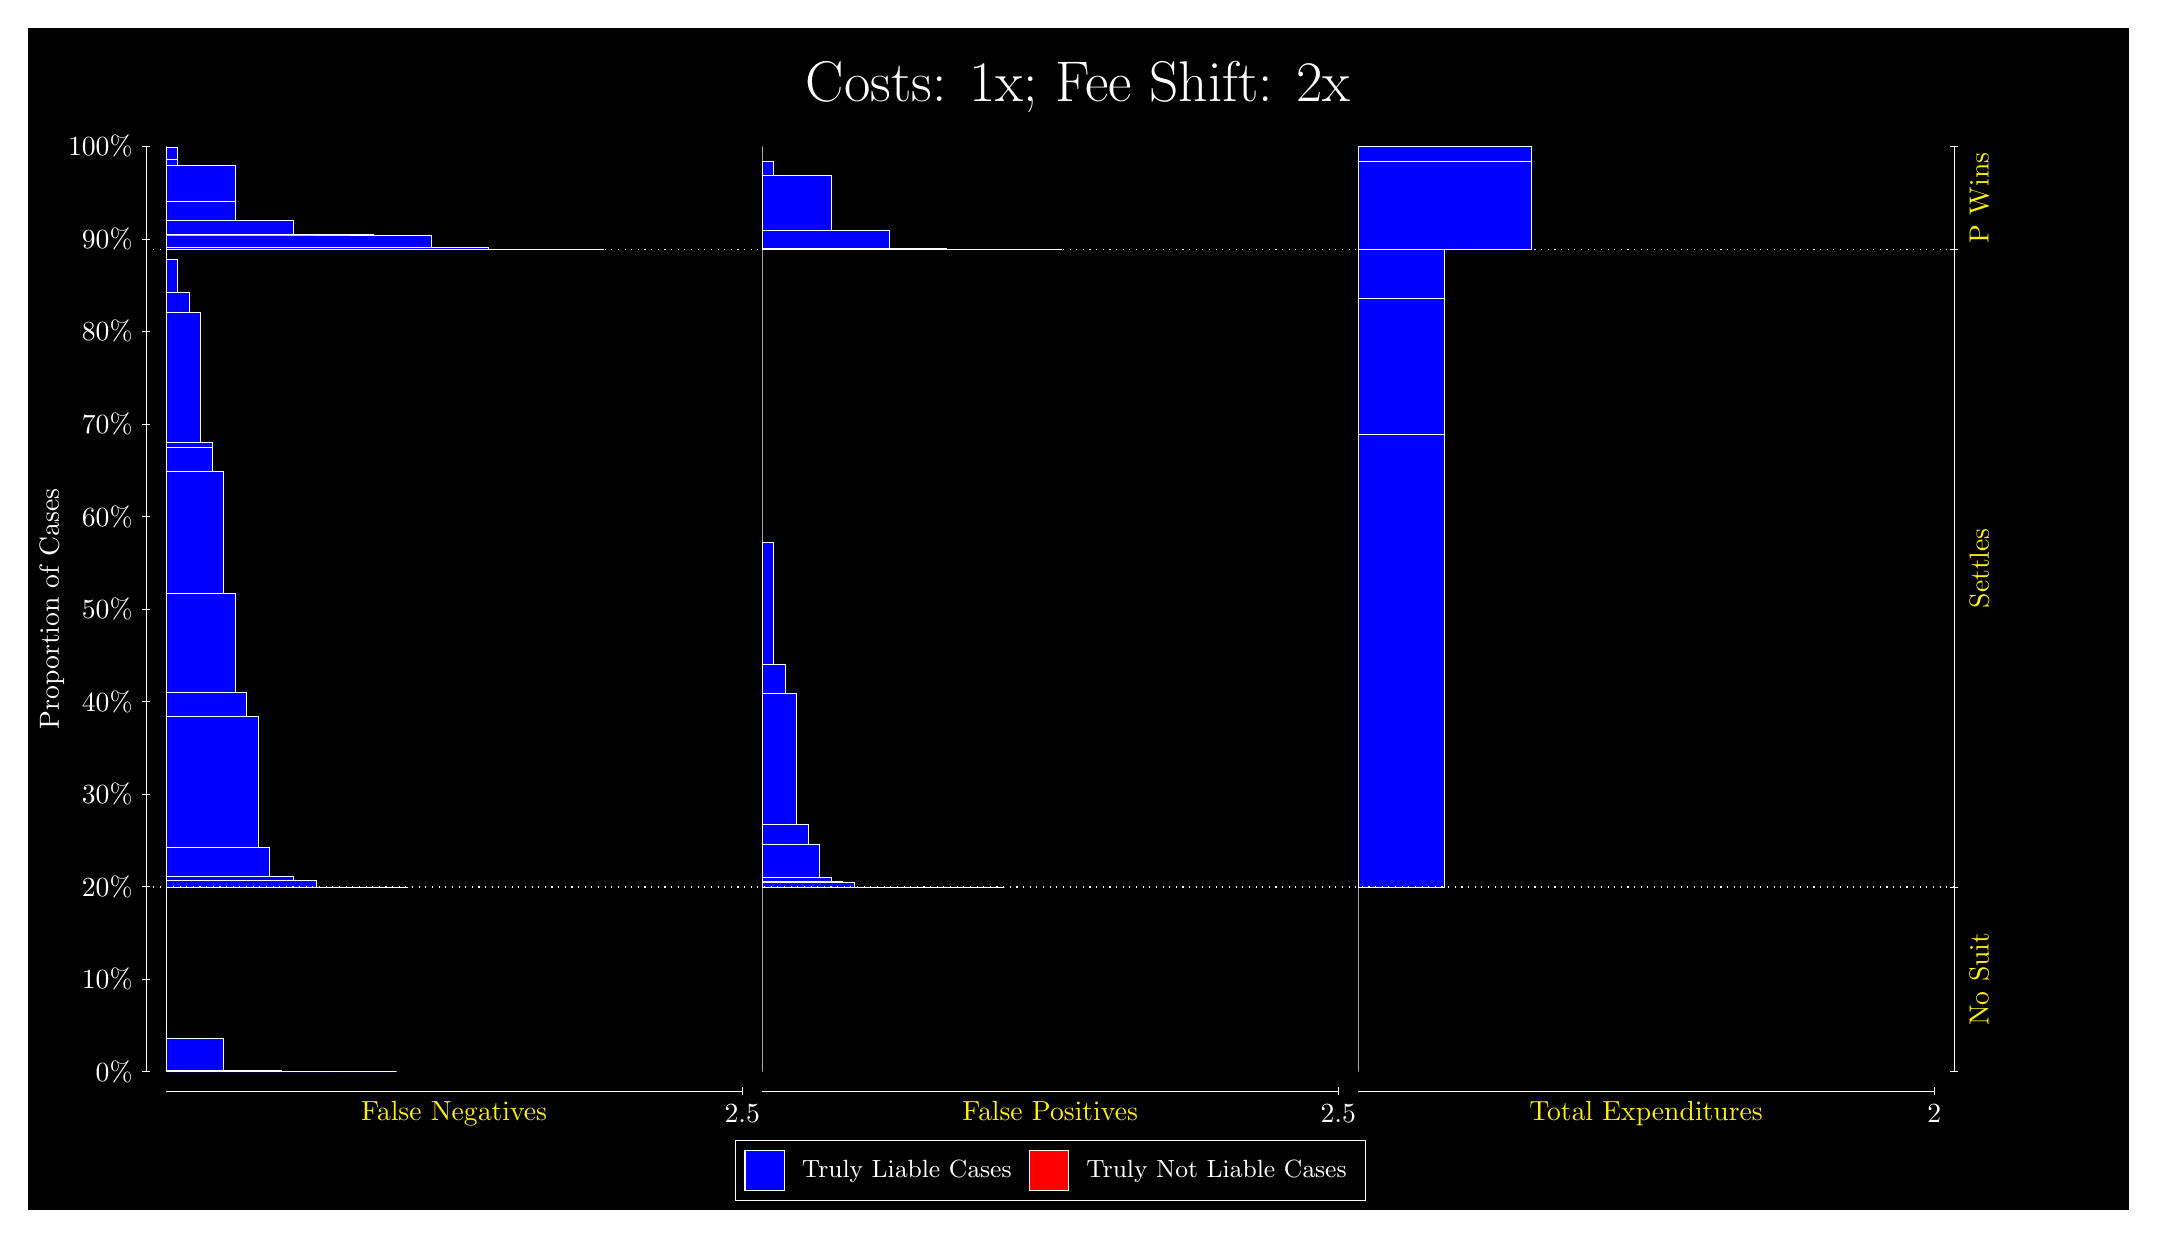
\begin{tikzpicture}
\draw[fill=black] (0,0) rectangle (26.667,15);
\draw[text=white] (0,13.5) rectangle (26.667,15) node[midway] {\huge Costs: 1x; Fee Shift: 2x};
\draw[white, very thin] (1.5,1.75) -- (1.5,13.5);
\node[rotate=90, text=white, anchor=center] at (0.3, 7.625) {Proportion of Cases};
\draw[white, very thin] (1.45,1.75) -- (1.55,1.75);
\node[text=white, anchor=east] at (1.45, 1.75) {0\%};
\draw[white, very thin] (1.45,2.925) -- (1.55,2.925);
\node[text=white, anchor=east] at (1.45, 2.925) {10\%};
\draw[white, very thin] (1.45,4.1) -- (1.55,4.1);
\node[text=white, anchor=east] at (1.45, 4.1) {20\%};
\draw[white, very thin] (1.45,5.275) -- (1.55,5.275);
\node[text=white, anchor=east] at (1.45, 5.275) {30\%};
\draw[white, very thin] (1.45,6.45) -- (1.55,6.45);
\node[text=white, anchor=east] at (1.45, 6.45) {40\%};
\draw[white, very thin] (1.45,7.625) -- (1.55,7.625);
\node[text=white, anchor=east] at (1.45, 7.625) {50\%};
\draw[white, very thin] (1.45,8.8) -- (1.55,8.8);
\node[text=white, anchor=east] at (1.45, 8.8) {60\%};
\draw[white, very thin] (1.45,9.975) -- (1.55,9.975);
\node[text=white, anchor=east] at (1.45, 9.975) {70\%};
\draw[white, very thin] (1.45,11.15) -- (1.55,11.15);
\node[text=white, anchor=east] at (1.45, 11.15) {80\%};
\draw[white, very thin] (1.45,12.325) -- (1.55,12.325);
\node[text=white, anchor=east] at (1.45, 12.325) {90\%};
\draw[white, very thin] (1.45,13.5) -- (1.55,13.5);
\node[text=white, anchor=east] at (1.45, 13.5) {100\%};

\draw[white, very thin] (24.457,1.75) -- (24.457,13.5);
\draw[white, very thin] (24.407,1.75) -- (24.507,1.75);
\node[anchor=west] at (24.407, 1.75) {};
\draw[white, very thin] (24.407,4.0929) -- (24.507,4.0929);
\node[anchor=west] at (24.407, 4.0929) {};
\draw[white, very thin] (24.407,12.192) -- (24.507,12.192);
\node[anchor=west] at (24.407, 12.192) {};
\draw[white, very thin] (24.407,13.5) -- (24.507,13.5);
\node[anchor=west] at (24.407, 13.5) {};

\draw[white, very thin, fill=blue] (1.75,1.75) rectangle (4.6775,1.75);
\draw[white, very thin, fill=blue] (1.75,1.75) rectangle (3.9457,1.7501);
\draw[white, very thin, fill=blue] (1.75,1.7501) rectangle (3.2138,1.7629);
\draw[white, very thin, fill=blue] (1.75,1.7629) rectangle (2.4819,2.1747);
\draw[white, very thin, fill=red] (1.75,2.1747) rectangle (1.75,2.1747);
\draw[white, very thin, fill=blue] (1.75,2.1747) rectangle (1.75,4.0929);
\draw[white, very thin, fill=blue] (1.75,4.0929) rectangle (4.8239,4.0929);
\draw[white, very thin, fill=blue] (1.75,4.0929) rectangle (4.5312,4.0929);
\draw[white, very thin, fill=blue] (1.75,4.0929) rectangle (4.2384,4.0929);
\draw[white, very thin, fill=blue] (1.75,4.0929) rectangle (4.092,4.0929);
\draw[white, very thin, fill=blue] (1.75,4.0929) rectangle (3.7993,4.0929);
\draw[white, very thin, fill=blue] (1.75,4.0929) rectangle (3.6529,4.1765);
\draw[white, very thin, fill=blue] (1.75,4.1765) rectangle (3.5065,4.1791);
\draw[white, very thin, fill=blue] (1.75,4.1791) rectangle (3.3602,4.2332);
\draw[white, very thin, fill=blue] (1.75,4.2332) rectangle (3.0674,4.5927);
\draw[white, very thin, fill=blue] (1.75,4.5927) rectangle (3.0674,4.5958);
\draw[white, very thin, fill=blue] (1.75,4.5958) rectangle (2.921,6.259);
\draw[white, very thin, fill=blue] (1.75,6.259) rectangle (2.7746,6.5614);
\draw[white, very thin, fill=blue] (1.75,6.5614) rectangle (2.6283,7.8196);
\draw[white, very thin, fill=blue] (1.75,7.8196) rectangle (2.4819,9.3668);
\draw[white, very thin, fill=blue] (1.75,9.3668) rectangle (2.3355,9.6782);
\draw[white, very thin, fill=blue] (1.75,9.6782) rectangle (2.3355,9.7363);
\draw[white, very thin, fill=blue] (1.75,9.7363) rectangle (2.1891,11.395);
\draw[white, very thin, fill=blue] (1.75,11.395) rectangle (2.0428,11.644);
\draw[white, very thin, fill=blue] (1.75,11.644) rectangle (1.8964,12.066);
\draw[white, very thin, fill=red] (1.75,12.066) rectangle (1.75,12.066);
\draw[white, very thin, fill=blue] (1.75,12.066) rectangle (1.75,12.192);
\draw[white, very thin, fill=blue] (1.75,12.192) rectangle (7.3123,12.192);
\draw[white, very thin, fill=blue] (1.75,12.192) rectangle (6.5805,12.192);
\draw[white, very thin, fill=blue] (1.75,12.192) rectangle (5.8486,12.217);
\draw[white, very thin, fill=blue] (1.75,12.217) rectangle (5.1167,12.369);
\draw[white, very thin, fill=blue] (1.75,12.369) rectangle (4.8239,12.369);
\draw[white, very thin, fill=blue] (1.75,12.369) rectangle (4.3848,12.379);
\draw[white, very thin, fill=blue] (1.75,12.379) rectangle (4.092,12.379);
\draw[white, very thin, fill=blue] (1.75,12.379) rectangle (3.6529,12.379);
\draw[white, very thin, fill=blue] (1.75,12.379) rectangle (3.3602,12.559);
\draw[white, very thin, fill=blue] (1.75,12.559) rectangle (2.921,12.559);
\draw[white, very thin, fill=blue] (1.75,12.559) rectangle (2.6283,12.797);
\draw[white, very thin, fill=blue] (1.75,12.797) rectangle (2.6283,13.264);
\draw[white, very thin, fill=blue] (1.75,13.264) rectangle (1.8964,13.338);
\draw[white, very thin, fill=blue] (1.75,13.338) rectangle (1.8964,13.486);
\draw[white, very thin, fill=red] (1.75,13.486) rectangle (1.75,13.486);
\draw[white, very thin, fill=blue] (1.75,13.486) rectangle (1.75,13.5);
\draw[white, very thin, fill=red] (9.3189,1.75) rectangle (9.3189,1.75);
\draw[white, very thin, fill=blue] (9.3189,1.75) rectangle (9.3189,4.0929);
\draw[white, very thin, fill=red] (9.3189,4.0929) rectangle (12.393,4.0929);
\draw[white, very thin, fill=blue] (9.3189,4.0929) rectangle (12.393,4.0929);
\draw[white, very thin, fill=red] (9.3189,4.0929) rectangle (11.807,4.0929);
\draw[white, very thin, fill=blue] (9.3189,4.0929) rectangle (11.807,4.0929);
\draw[white, very thin, fill=blue] (9.3189,4.0929) rectangle (11.661,4.0929);
\draw[white, very thin, fill=red] (9.3189,4.0929) rectangle (11.222,4.0929);
\draw[white, very thin, fill=blue] (9.3189,4.0929) rectangle (11.222,4.0929);
\draw[white, very thin, fill=blue] (9.3189,4.0929) rectangle (11.075,4.0929);
\draw[white, very thin, fill=blue] (9.3189,4.0929) rectangle (10.929,4.0929);
\draw[white, very thin, fill=red] (9.3189,4.0929) rectangle (10.636,4.0929);
\draw[white, very thin, fill=blue] (9.3189,4.0929) rectangle (10.636,4.0936);
\draw[white, very thin, fill=blue] (9.3189,4.0936) rectangle (10.49,4.1529);
\draw[white, very thin, fill=red] (9.3189,4.1529) rectangle (10.344,4.1529);
\draw[white, very thin, fill=blue] (9.3189,4.1529) rectangle (10.344,4.16);
\draw[white, very thin, fill=blue] (9.3189,4.16) rectangle (10.197,4.2183);
\draw[white, very thin, fill=red] (9.3189,4.2183) rectangle (10.051,4.2183);
\draw[white, very thin, fill=blue] (9.3189,4.2183) rectangle (10.051,4.6412);
\draw[white, very thin, fill=blue] (9.3189,4.6412) rectangle (9.9044,4.8898);
\draw[white, very thin, fill=blue] (9.3189,4.8898) rectangle (9.758,6.5485);
\draw[white, very thin, fill=blue] (9.3189,6.5485) rectangle (9.6116,6.9179);
\draw[white, very thin, fill=blue] (9.3189,6.9179) rectangle (9.4652,8.4651);
\draw[white, very thin, fill=blue] (9.3189,8.4651) rectangle (9.3189,12.192);
\draw[white, very thin, fill=red] (9.3189,12.192) rectangle (13.125,12.192);
\draw[white, very thin, fill=blue] (9.3189,12.192) rectangle (13.125,12.192);
\draw[white, very thin, fill=red] (9.3189,12.192) rectangle (12.393,12.192);
\draw[white, very thin, fill=blue] (9.3189,12.192) rectangle (12.393,12.192);
\draw[white, very thin, fill=red] (9.3189,12.192) rectangle (11.661,12.192);
\draw[white, very thin, fill=blue] (9.3189,12.192) rectangle (11.661,12.206);
\draw[white, very thin, fill=red] (9.3189,12.206) rectangle (10.929,12.206);
\draw[white, very thin, fill=blue] (9.3189,12.206) rectangle (10.929,12.428);
\draw[white, very thin, fill=blue] (9.3189,12.428) rectangle (10.197,13.133);
\draw[white, very thin, fill=red] (9.3189,13.133) rectangle (9.9044,13.133);
\draw[white, very thin, fill=blue] (9.3189,13.133) rectangle (9.9044,13.133);
\draw[white, very thin, fill=blue] (9.3189,13.133) rectangle (9.4652,13.312);
\draw[white, very thin, fill=red] (9.3189,13.312) rectangle (9.3189,13.312);
\draw[white, very thin, fill=blue] (9.3189,13.312) rectangle (9.3189,13.5);
\draw[white, very thin, fill=red] (16.888,1.75) rectangle (16.888,1.75);
\draw[white, very thin, fill=blue] (16.888,1.75) rectangle (16.888,4.0929);
\draw[white, very thin, fill=red] (16.888,4.0929) rectangle (17.986,4.0929);
\draw[white, very thin, fill=blue] (16.888,4.0929) rectangle (17.986,9.8367);
\draw[white, very thin, fill=red] (16.888,9.8367) rectangle (17.986,9.8367);
\draw[white, very thin, fill=blue] (16.888,9.8367) rectangle (17.986,11.572);
\draw[white, very thin, fill=red] (16.888,11.572) rectangle (17.986,11.572);
\draw[white, very thin, fill=blue] (16.888,11.572) rectangle (17.986,12.192);
\draw[white, very thin, fill=red] (16.888,12.192) rectangle (19.083,12.192);
\draw[white, very thin, fill=blue] (16.888,12.192) rectangle (19.083,13.312);
\draw[white, very thin, fill=red] (16.888,13.312) rectangle (19.083,13.312);
\draw[white, very thin, fill=blue] (16.888,13.312) rectangle (19.083,13.5);
\draw[white, dotted] (1.5,4.0929) -- (24.457,4.0929);
\draw[white, dotted] (1.5,12.192) -- (24.457,12.192);
\draw[white, very thin] (1.75,1.5) -- (9.0689,1.5);
\node[text=yellow, anchor=north] at (5.4094, 1.5) {False Negatives};
\draw[white, very thin] (9.0689,1.45) -- (9.0689,1.55);
\node[text=white, anchor=north] at (9.0689, 1.45) {2.5};

\draw[white, very thin] (9.3189,1.5) -- (16.638,1.5);
\node[text=yellow, anchor=north] at (12.978, 1.5) {False Positives};
\draw[white, very thin] (16.638,1.45) -- (16.638,1.55);
\node[text=white, anchor=north] at (16.638, 1.45) {2.5};

\draw[white, very thin] (16.888,1.5) -- (24.207,1.5);
\node[text=yellow, anchor=north] at (20.547, 1.5) {Total Expenditures};
\draw[white, very thin] (24.207,1.45) -- (24.207,1.55);
\node[text=white, anchor=north] at (24.207, 1.45) {2};

\node[text=yellow, centered, rotate=90] at (24.777, 2.9215) {No Suit};
\node[text=yellow, centered, rotate=90] at (24.777, 8.1424) {Settles};
\node[text=yellow, centered, rotate=90] at (24.777, 12.846) {P Wins};

\draw (12.978300999999998,1.5) node[draw=none] (baseCoordinate) {};
\begin{scope}[align=center]
        \matrix[scale=0.5, draw=white, below=0.5cm of baseCoordinate, nodes={draw}, column sep=0.1cm]{
            \node[rectangle, draw, minimum width=0.5cm, minimum height=0.5cm, fill=blue] {}; &
            \node[draw=none, font=\small, text=white] (B) {Truly Liable Cases}; &
            \node[rectangle, draw, minimum width=0.5cm, minimum height=0.5cm, fill=red] {}; &
            \node[draw=none, font=\small, text=white] (B) {Truly Not Liable Cases}; \\
            };
\end{scope}

\end{tikzpicture}
\end{document}